\documentclass[11pt]{article}
\usepackage[margin=1in]{geometry}
\usepackage{graphicx, booktabs, hyperref, xcolor, parskip, amsmath}

\begin{document}

\begin{center}
{\Large \textbf{Experiment Results:\\Concordia Agents in the Repeated Prisoner's Dilemma}}\\[0.5em]
{\large February 2026 \quad $\cdot$ \quad Status: Post-analysis (v2: pre/post comparison)}
\end{center}

%% --- 1. RESEARCH QUESTION ---
\section*{Research Question}

How do LLM-based agents with associative memory and goal-oriented reasoning behave in a finitely repeated Prisoner's Dilemma? Standard game theory predicts mutual defection via backward induction in a finitely repeated PD, yet behavioral experiments with humans routinely find substantial cooperation, particularly in early and middle rounds, with unraveling toward defection near the end (``endgame effect''). This experiment tests whether Concordia's \texttt{RationalEntity} agents---which combine situation perception, memory retrieval, option evaluation, and goal-directed reasoning---produce human-like cooperation patterns or converge to the Nash equilibrium.

\textbf{Secondary question (v2):} Does the implementation of ``simultaneous'' moves matter? The initial run (``pre-fix'') used a fixed act order (A always first) and shared observation labels (``Player A chose X, Player B chose Y''). The post-fix run randomizes act order each round and uses role-relative observations (``You chose X. The other player chose Y.''). We compare the two conditions to determine whether the positional asymmetry found in v1 was an implementation artifact.

%% --- 2. EXPERIMENTAL DESIGN ---
\section*{Experimental Design}

\textbf{Game:} Repeated Prisoner's Dilemma, 10 rounds, 2 symmetric players (Player A and Player B).

\textbf{Actions:} Each round, both players simultaneously choose COOPERATE or DEFECT.

\textbf{Payoff matrix (per round):}

\begin{center}
\begin{tabular}{lcc}
\toprule
 & B Cooperates & B Defects \\
\midrule
A Cooperates & \$3 / \$3 & \$0 / \$5 \\
A Defects & \$5 / \$0 & \$1 / \$1 \\
\bottomrule
\end{tabular}
\end{center}

Maximum possible per-player earnings: \$30 (mutual cooperation all 10 rounds). Mutual defection benchmark: \$10.

\textbf{Agent architecture:} Concordia \texttt{RationalEntity} prefab with components: Instructions $\to$ Observation $\to$ SituationPerception $\to$ RelevantMemories $\to$ AvailableOptionsPerception $\to$ BestOptionPerception $\to$ ConcatAct. Each agent's goal string specifies the payoff matrix and earnings-maximization objective with no prescribed strategy.

\textbf{Model:} \texttt{gpt-4o-mini}. N = 30 sessions per condition.

\textbf{Conditions:}
\begin{enumerate}
\item \textbf{Pre-fix} (seed 42): Fixed act order (A always first), shared observation labels referencing ``Player A'' and ``Player B'' by name.
\item \textbf{Post-fix} (seed 43): Randomized act order each round (\texttt{random.choice([True, False])}), role-relative observations (``You chose X. The other player chose Y.'').
\end{enumerate}

%% --- 3. DATA OVERVIEW ---
\section*{Data Overview}

\textbf{Sample:} 60 simulations (30 pre-fix + 30 post-fix), 600 total rounds. No sessions excluded---all completed 10 rounds with valid outputs. Zero invalid actions across all 600 rounds.

\textbf{Summary statistics by condition:}

\begin{center}
\begin{tabular}{l rr rr}
\toprule
 & \multicolumn{2}{c}{Pre-fix} & \multicolumn{2}{c}{Post-fix} \\
Metric & Mean & SD & Mean & SD \\
\midrule
A earnings (\$) & 22.3 & 9.7 & 22.9 & 7.3 \\
B earnings (\$) & 26.3 & 4.6 & 22.6 & 7.5 \\
Joint earnings (\$) & 48.6 & 13.8 & 45.5 & 12.7 \\
Efficiency & 0.81 & 0.23 & 0.76 & 0.21 \\
A cooperation rate & 0.71 & 0.34 & 0.59 & 0.37 \\
B cooperation rate & 0.63 & 0.44 & 0.60 & 0.37 \\
Mutual coop rounds & 5.9 & 4.8 & 5.0 & 4.5 \\
Full coop games & \multicolumn{2}{c}{16/30 (53\%)} & \multicolumn{2}{c}{6/30 (20\%)} \\
A exploits B & 0.4 & 1.0 & 0.9 & 1.3 \\
B exploits A & 1.2 & 1.6 & 0.9 & 1.2 \\
\bottomrule
\end{tabular}
\end{center}

%% --- 4. RESULTS ---
\section*{Results}

\subsection*{Primary Outcome: Asymmetry Eliminated}

The pre-fix condition showed a significant B $>$ A earnings asymmetry: Player B earned \$4.0 more on average (paired $t(29) = -3.45$, $p = 0.002$). The post-fix condition \emph{eliminated} this asymmetry entirely: the A$-$B gap was $+$\$0.3 ($t(29) = 0.25$, $p = 0.81$).

The between-condition comparison of the A$-$B earnings gap is significant: $t(58) = -2.43$, $p = 0.018$. This confirms that the asymmetry was a \textbf{positional artifact} caused by (a) A always acting first and (b) non-relative observation labels, not by statistical noise or inherent agent asymmetry.

The exploitation rates tell the same story: pre-fix B exploited A 3$\times$ more often than A exploited B (1.2 vs.\ 0.4 rounds/game). Post-fix, exploitation is symmetric (0.9 vs.\ 0.9).

\begin{figure}[h]
\centering
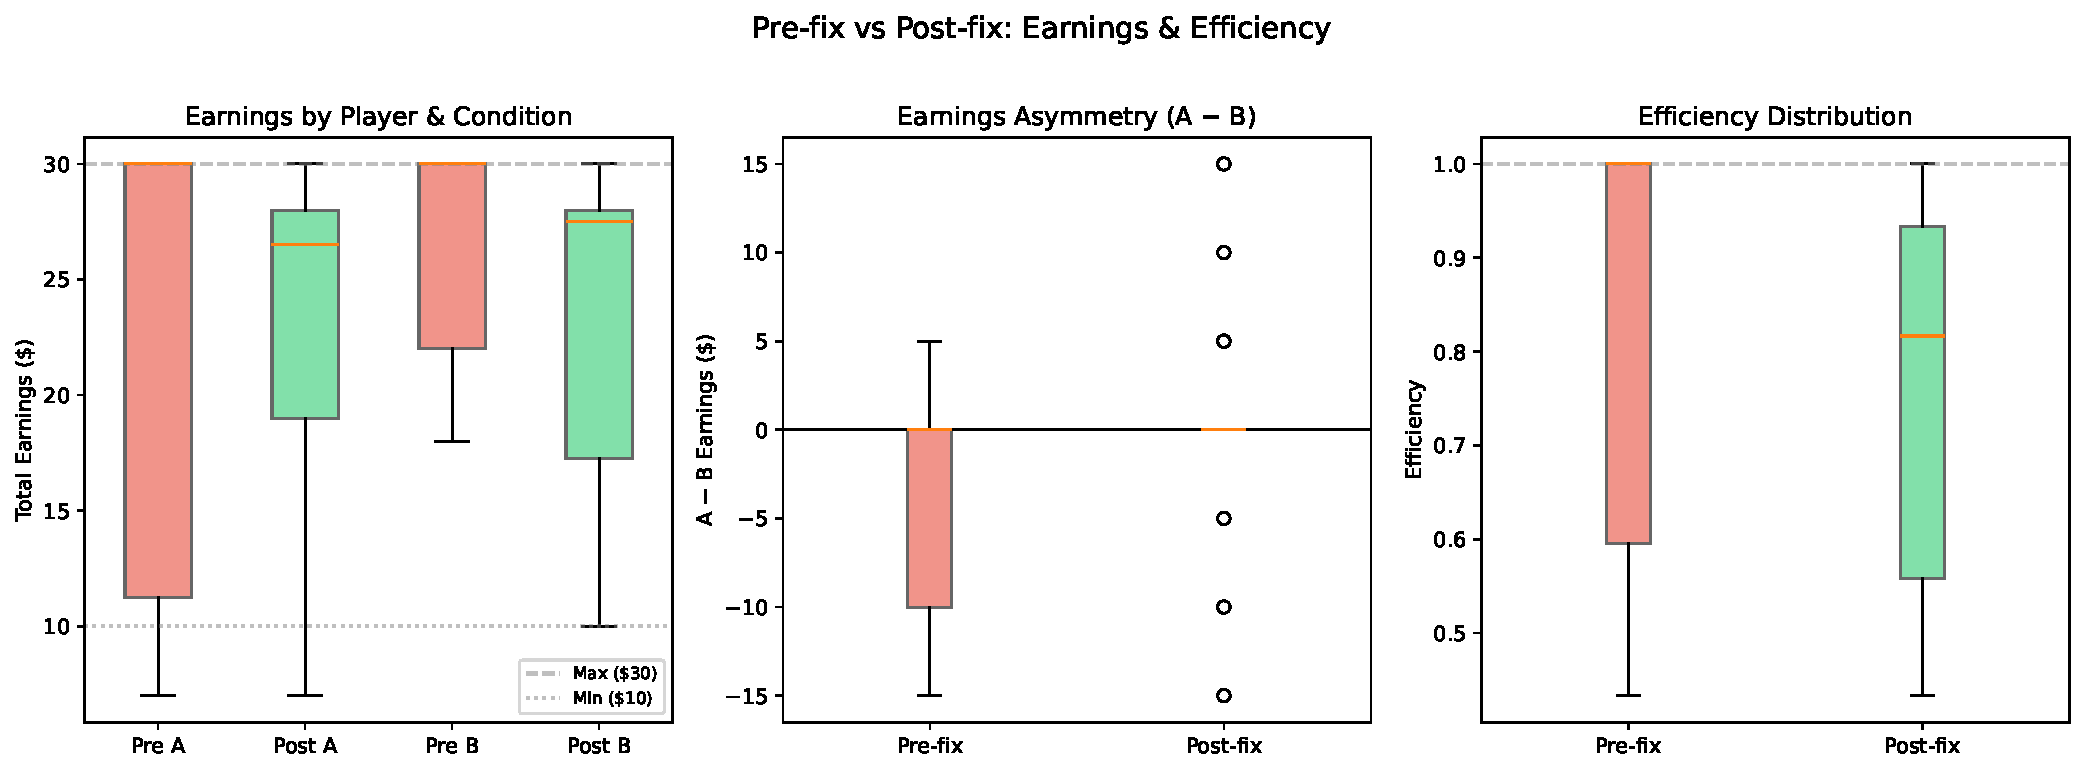
\includegraphics[width=0.95\textwidth]{plots/v2_earnings_comparison.pdf}
\caption{Left: Earnings by player and condition (pre-fix B $>$ A gap visible; post-fix symmetric). Center: A$-$B earnings gap (pre-fix significantly negative; post-fix centered on zero). Right: Efficiency (slightly lower post-fix but not significant).}
\end{figure}

\subsection*{Secondary Outcome: Cooperation Rate Declined}

An unexpected finding: the post-fix condition shows \emph{lower} cooperation and fewer full-cooperation games. Full cooperation dropped from 53\% (16/30) to 20\% (6/30), a significant difference (Fisher's exact $p = 0.015$).

However, the \emph{average} cooperation rates are not significantly different: A coop rate 0.71 vs.\ 0.59 ($t = 1.35$, $p = 0.18$), B coop rate 0.63 vs.\ 0.60 ($t = 0.35$, $p = 0.73$). The difference is driven by the tail of the distribution: the pre-fix condition had a large cluster of perfect-cooperation games that partially disappeared post-fix.

Mean efficiency also declined from 81\% to 76\%, but this is not significant ($t = 0.89$, $p = 0.37$).

\begin{figure}[h]
\centering
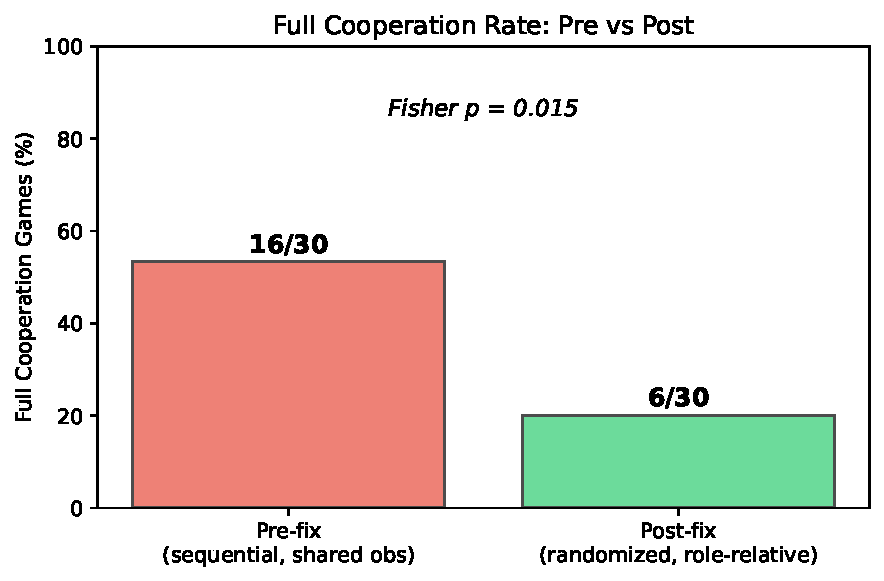
\includegraphics[width=0.75\textwidth]{plots/v2_full_coop_rate.pdf}
\caption{Full cooperation rate by condition. The drop from 53\% to 20\% is significant (Fisher's exact $p = 0.015$).}
\end{figure}

\subsection*{Round-by-Round Dynamics}

\begin{center}
\begin{tabular}{c rrrr}
\toprule
Round & Pre A & Post A & Pre B & Post B \\
\midrule
1 & 80\% & 40\% & 70\% & 47\% \\
2 & 67\% & 50\% & 57\% & 57\% \\
3 & 73\% & 67\% & 63\% & 73\% \\
4 & 67\% & 67\% & 67\% & 57\% \\
5 & 70\% & 60\% & 60\% & 63\% \\
6 & 77\% & 57\% & 67\% & 63\% \\
7 & 73\% & 60\% & 60\% & 57\% \\
8 & 73\% & 67\% & 63\% & 60\% \\
9 & 70\% & 63\% & 63\% & 60\% \\
10 & 63\% & 60\% & 63\% & 60\% \\
\bottomrule
\end{tabular}
\end{center}

The most striking difference is in \textbf{Round 1}: pre-fix A cooperated 80\% vs.\ post-fix A cooperated only 40\%. This 40-percentage-point drop in first-round cooperation for A suggests that the pre-fix condition's fixed act-order (A always first) somehow encouraged A to open with cooperation, possibly because A's initial move was ``fresher'' in the LLM context. Post-fix, with randomized ordering and role-relative framing, first-round cooperation is closer to 50/50 for both players.

Neither condition shows an endgame effect---cooperation rates remain roughly flat from round 2 onward.

\begin{figure}[h]
\centering
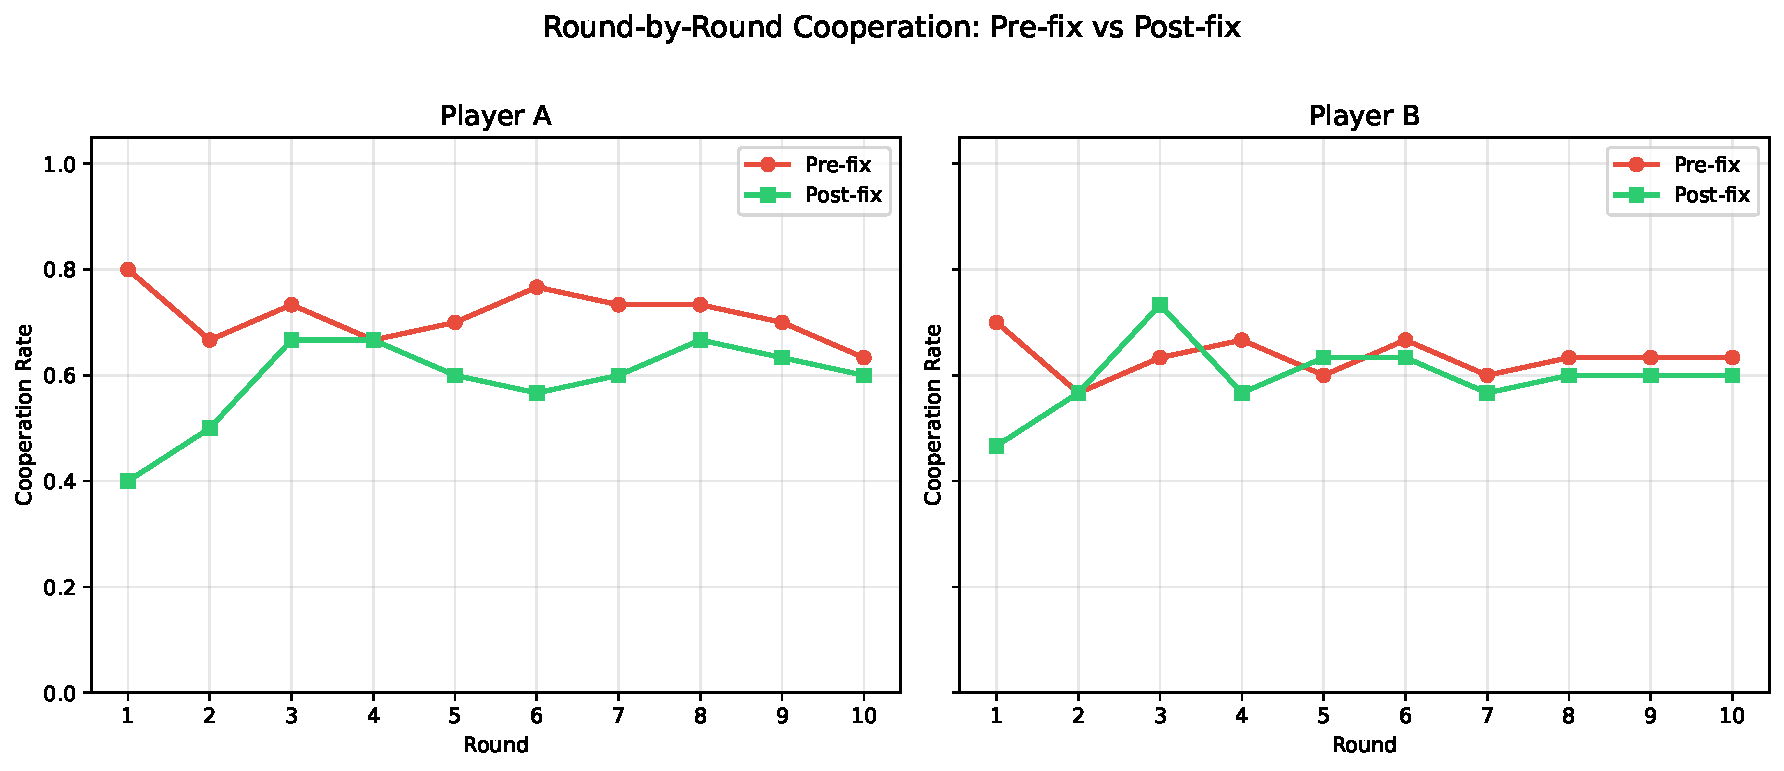
\includegraphics[width=0.95\textwidth]{plots/v2_cooperation_comparison.pdf}
\caption{Round-by-round cooperation rates. Pre-fix (red) vs.\ post-fix (green). The largest gap is in Round 1 for Player A.}
\end{figure}

\subsection*{Choice Sequence Patterns}

\begin{figure}[h]
\centering
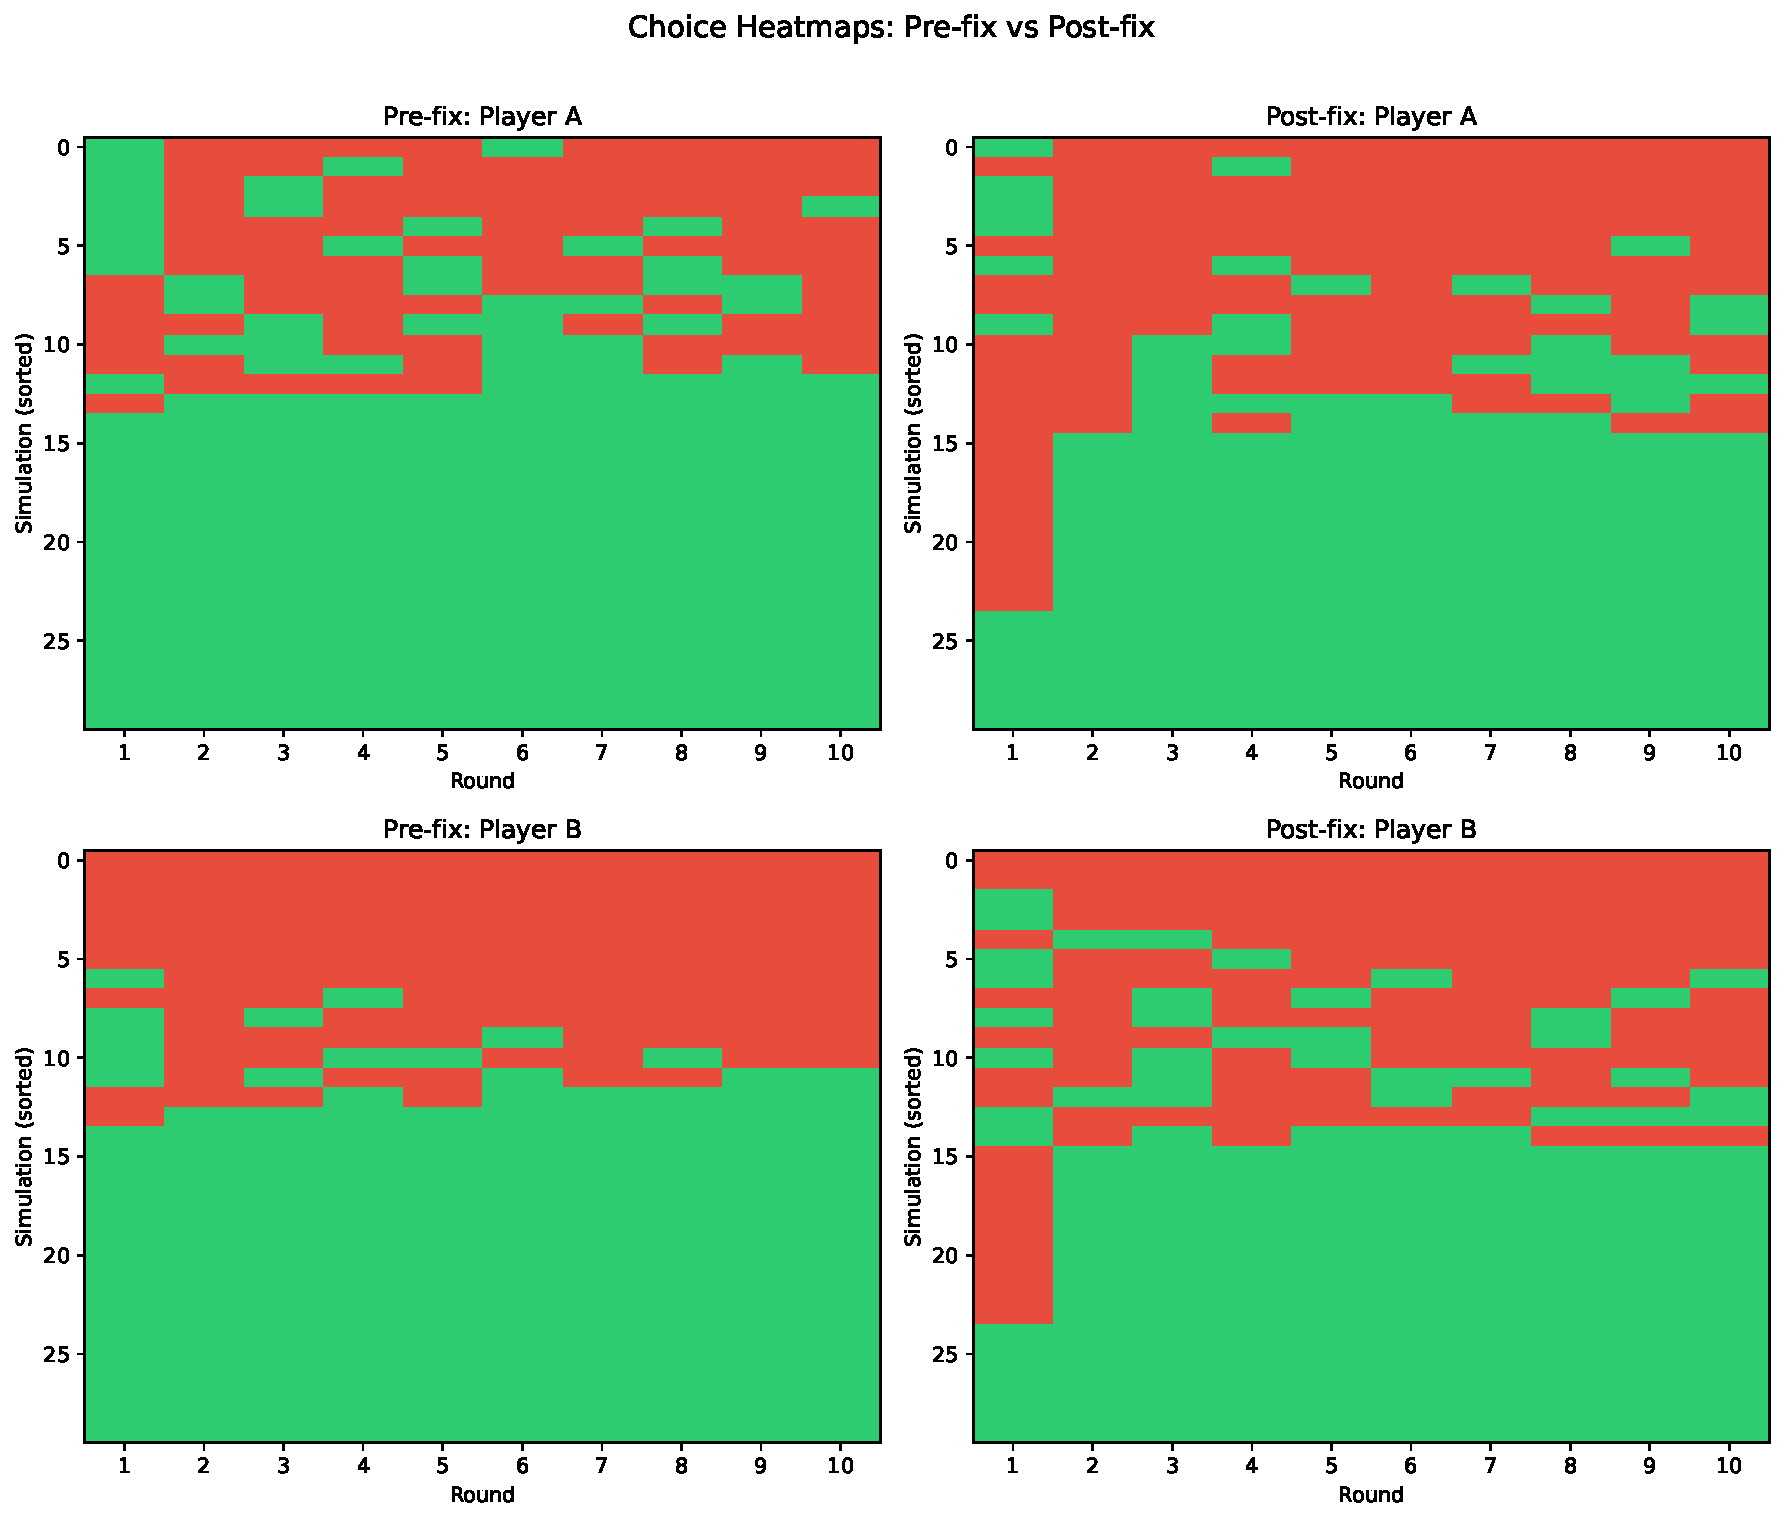
\includegraphics[width=0.95\textwidth]{plots/v2_choice_heatmap.pdf}
\caption{Choice heatmaps (green = cooperate, red = defect). Top row: Player A; bottom row: Player B. Left: pre-fix; right: post-fix. Simulations sorted by total cooperation. The post-fix condition has fewer ``solid green'' rows (full cooperation games).}
\end{figure}

The heatmaps confirm the bimodal pattern persists in both conditions but with different proportions. Pre-fix had roughly a 50/50 split between full cooperators and defectors. Post-fix shifted to roughly 20/80, with more mixed-strategy games and fewer lock-in cooperators.

%% --- 5. EVALUATION ---
\section*{Evaluation}

\subsection*{Did We Learn Something Interesting?}

\textbf{Yes---two clear findings:}

\begin{enumerate}
\item \textbf{The B $>$ A asymmetry was entirely an implementation artifact.} The combination of fixed act-order and named observation labels created a systematic advantage for Player B. Randomizing act-order and using role-relative observations eliminated the asymmetry completely ($p = 0.018$ for the between-condition difference). \textbf{Methodological lesson:} In Concordia simulations of simultaneous-move games, both act-order randomization and role-relative observations are necessary. This should be standard practice.

\item \textbf{Implementation details affect cooperation rates substantially.} The post-fix condition dropped full cooperation from 53\% to 20\% ($p = 0.015$), driven primarily by a collapse in Round 1 cooperation for Player A (80\% $\to$ 40\%). This means the high cooperation rate in the pre-fix condition was \emph{partially inflated} by the positional bias. The ``true'' cooperation rate under fair conditions is closer to 59--60\%, with 20\% of games achieving full cooperation---still well above the Nash equilibrium of 0\%, but less dramatic than the initial 53\% figure.
\end{enumerate}

\textbf{The corrected picture:} Concordia \texttt{RationalEntity} agents cooperate at $\sim$60\% in a 10-round PD with no endgame effect. Full cooperation occurs in $\sim$20\% of games. The bimodal pattern (cooperate from start or defect from start) persists. Both findings diverge from Nash predictions and from typical human behavior (where cooperation starts high and decays).

\subsection*{Limitations}

\begin{itemize}
\item \textbf{Confounded comparison:} The pre-fix and post-fix runs changed \emph{two things simultaneously}---act order randomization and role-relative observations. We cannot determine which change drove the cooperation decline (or whether both contributed). A 2$\times$2 factorial with (act order: fixed vs.\ random) $\times$ (observations: named vs.\ relative) would disentangle these.
\item \textbf{Different seeds:} Pre-fix used seed 42, post-fix used seed 43. While 30 simulations per condition provides reasonable power, the different seeds mean some variance is attributable to sampling.
\item \textbf{Single model (gpt-4o-mini):} Results may not generalize to other models.
\item \textbf{No human baseline:} We cannot say whether 60\% cooperation is ``human-like'' without running the same game with human subjects.
\end{itemize}

%% --- 6. NEXT EXPERIMENT ---
\section*{Next Experiment}

\textbf{Recommended archetype: DEEPEN}

The corrected post-fix results provide a clean baseline: $\sim$60\% cooperation, no endgame effect, bimodal pattern, symmetric earnings. The next experiment should test whether a well-studied manipulation from behavioral economics---\emph{costly punishment}---shifts cooperation rates as predicted by human experiments.

\textbf{Proposed experiment: Costly Punishment}

After each round, each player can pay \$1 to reduce the other player's earnings by \$3 (standard altruistic punishment mechanism from Fehr \& G\"achter, 2002). The hypothesis is that punishment availability will increase cooperation by deterring defection, converting the bimodal distribution (20\% full coop, 80\% mixed/defect) into a more cooperative distribution.

\textbf{Conditions:}
\begin{enumerate}
\item \texttt{pd\_concordia} (baseline: this experiment, post-fix)
\item \texttt{pd\_concordia\_punish} (same game + punishment stage after each round)
\end{enumerate}

\textbf{Predictions:}
\begin{enumerate}
\item Full cooperation rate increases from 20\% to $>$50\%.
\item Mean cooperation rate increases from 60\% to $>$80\%.
\item Punishment is used primarily in early rounds to establish norms, then declines.
\end{enumerate}

\textbf{Alternative:} To cleanly disentangle the act-order vs.\ observation-format effects, run a 2$\times$2 factorial: (fixed act-order $\times$ named observations, fixed $\times$ relative, random $\times$ named, random $\times$ relative). This would confirm which implementation detail drives the cooperation difference.

\textbf{Next step:} Run \texttt{/create-concordia-game} for the punishment variant, or run \texttt{/hypothesize} with the punishment hypothesis to formalize it first.

\subsection*{Prior Experiment Context (Machine-Readable)}
\begin{verbatim}
prior_hypothesis: LLM agents with structured cognitive architectures sustain
  non-trivial cooperation in a 10-round PD despite Nash prediction of defection
verdict: YES_INTERESTING
diagnosis: NA
key_finding: Asymmetry was implementation artifact (p=0.018);
  corrected cooperation ~60%, full coop 20%, no endgame effect;
  implementation details (act order, observation format) significantly
  affect cooperation rates (full coop 53% -> 20%, p=0.015)
key_statistic: post_fix_coop_rate=0.60, post_fix_full_coop=6/30=20%,
  asymmetry_eliminated (p=0.81), full_coop_decline (Fisher p=0.015)
dag_variables: X=cognitive_architecture, M=memory_and_reasoning,
  Y=cooperation_rate, Z=payoff_structure, W=implementation_details
testable_implications_results: cooperation>0=CONFIRMED,
  endgame_decline=REFUTED, symmetric_earnings=CONFIRMED_AFTER_FIX,
  implementation_neutral=REFUTED
next_archetype: DEEPEN
proposed_changes: Add costly punishment condition ($1 to punish,
  -$3 to target) to test whether punishment shifts cooperation
  from 20% full-coop to >50%
next_hypothesis_sketch: Costly punishment availability increases
  cooperation rate from 60% to >80% by deterring early defection,
  converting bimodal distribution to unimodal cooperative
\end{verbatim}

\end{document}
